\chapter{xSpark} \label{chap:xSpark}
%\begin{flushright}{\slshape    
%   Science, my boy, is made up of mistakes, but they are mistakes
%   which it is useful to make, because they lead little by little
%   to the truth}. \\ \medskip --- \citeauthor{verne_journey:1957}
%   \citetitle{verne_journey:1957} \citeyear{verne_journey:1957}
%\end{flushright} 
\lettrine[lines=4]{\textcolor{purple}{T}}{his} chapter illustrates the previous works done on xSpark, that is the base for the developments made and contribution given by this thesis.
%\section{xSpark}\label{sec:xSpark}
xSpark is a Spark extension that offers optimized and elastic provisioning of resources in order to meet execution deadlines. This is obtained by using nested control loops. A centralized control loop, implemented on the master node, controls the execution of the different stages of an application; at the same time multiple local loops, one per
executor, focus on task execution.
\begin{figure}
	\centering
	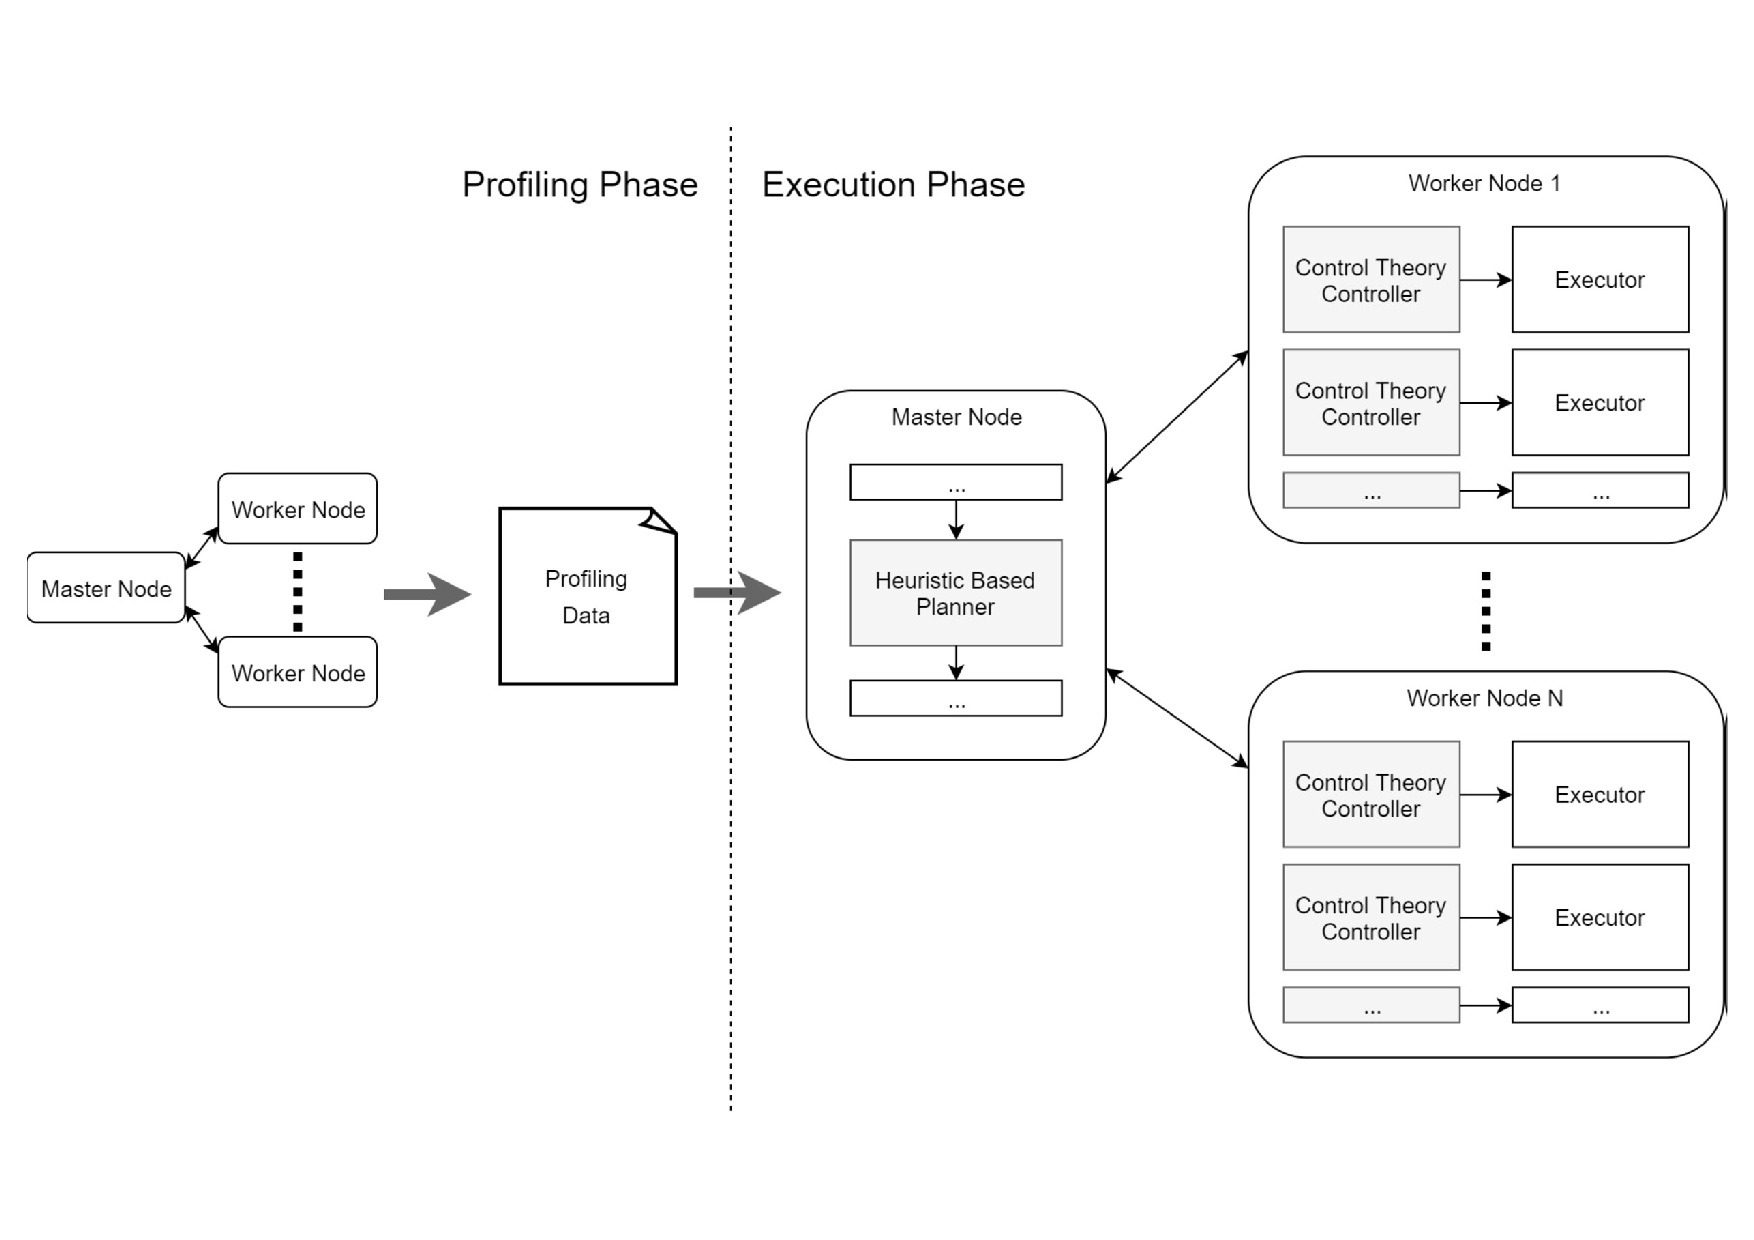
\includegraphics[width=\columnwidth]{Images/xspark_execution_flow.pdf}  
	\caption[xSpark high level setup and execution flow]{High level setup and execution flow of xSpark.}
	\label{fig:xSparkExecFlow}
\end{figure}

In \MyFig{fig:xSparkExecFlow} we can see a high level representation of xSpark execution flow. A preliminary Profiling Phase, that is executed once per application, is obtained by executing the application once to obtain information about its runtime execution. The log generated by the application are used to generate its Profiling Data.

In the Execution Phase, we control the application by means of xSpark’s control loops. 
The centralized control loop is represented as a Heuristic Based Planner, which exploits the profiling data, that are used to understand the amount of work that is needed to execute the application. This component uses the provided profiling data to determine the amount of resources to assign to executors for each of the application stages, in order to complete the execution within the given deadline. The local loops instead are represented as control theory controllers. They perform fine-grained tuning of the resources assigned to each of the executors using a control theory based controller. This component is used to counteract the possible imprecision of the estimated needed resources, which may be caused by different factors, such as the available memory, etc.

Usually Spark applications are run multiple times, as they are reusable and long lasting assets. xSpark exploits an initial profiling phase to create an enriched \textit{Directed Acyclic Graph} (DAG) ot \textit{Parallel Execution Plan} (\plan) describing the entire application execution flow, by collecting information about all the stages of the application. For each stage, xSpark annotates the DAG with the execution time (stage duration), the number of task processed, the number of input records read, the number of output record written and the nominal rate, defined as the number of records that a single core processes during one second of execution. 

%\lstinputlisting[
%firstline=1,
%lastline=19,
%float=tb,
%language=Python,
%tabsize=2,
%numbers=left,
%numberstyle=\tiny,
%stepnumber=1,
%numbersep=5pt,
%caption={Example of profiling data from a PageRank application.}, 
%captionpos=t,
%label=lst:profileFragment
%]{CodeFiles/profileFragment.json}

\begin{figure}
	\centering
	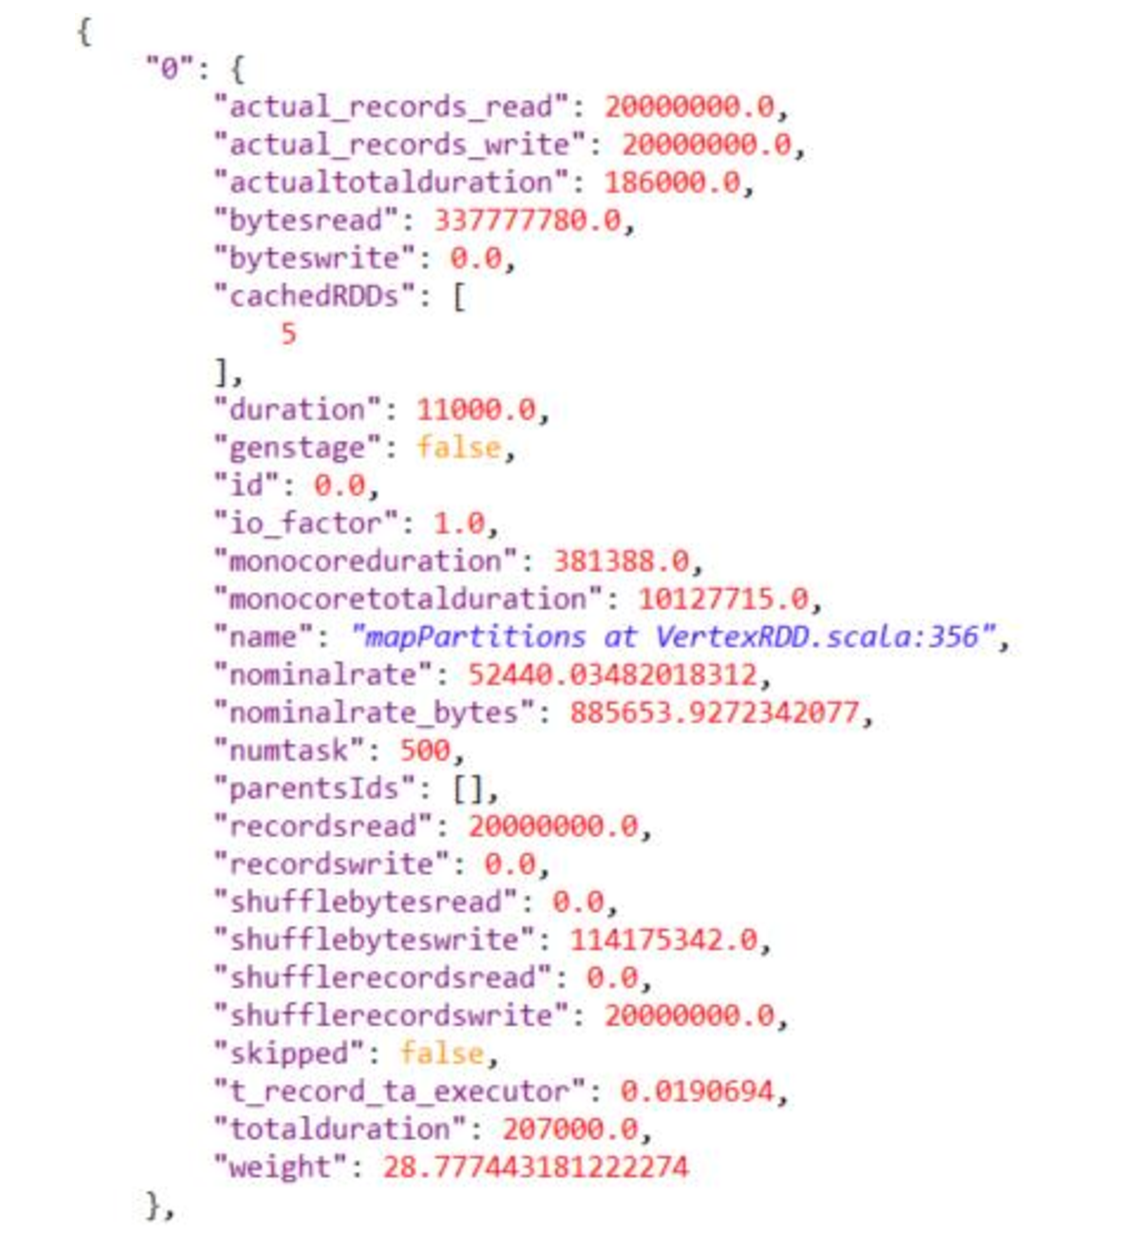
\includegraphics[width=\columnwidth]{Images/profile_fragment.pdf}  
	\caption[Example of profiling data from a Louvain application]{Example of profiling data from a Louvain application.}
	\label{fig:profileFragment}
\end{figure}

%In \MyListing{lst:profileFragment}
In \MyFig{fig:profileFragment} we can see a fragment, relative to stage number zero, of the profiling data of a Louvain application executed in xSpark.
The duration field contains the serialized total duration of the tasks in milliseconds.

At runtime, the a\plan allows the xSpark scheduler function to know how much
work was already completed and how much remains to be done. This means that xSpark can only optimize the allocation of the resources if all the executions of the same application use the same \plan. This might not always be the case, for example when the code contains branches or loops, because these might need to be resolved in different ways at runtime. If the application \plan at runtime differs from the one obtained during the profiling phase, xSpark is not able to estimate the amount of remaining work. 

The centralized control loop is activated before the execution of every stage, it uses a heuristic, explained in \MySec{sec:heuristic}, in order to assign a deadline to the stage, calculate the amount of CPU cores that are needed to satisfy it, and assign cores to the allocated executors. 

The per-stage deadline takes into account the amount of work already completed, the consumed time, and the overall deadline. All the computations done by the heuristic are based on the information stored in the \plan and obtained during the profiling phase. Unfortunately
many factors can influence the actual performance and invalidate the prediction, such as the amount of records that have been filtered-out, the available memory, the number of used nodes,
the storage layer dimension, and so on. It is important to remember that Spark mostly uses in-memory data, but there are operations like textFile, saveAsTextFile and saveAsSequenceFile that impose restricting constraints on the storage layer. If not correctly sized,
the storage layer might become a bottleneck, causing the throughput to degrade and thus making the provisioning predicted by xSpark incorrect.

Local control loops, explained in \MySec{subsec:controller}, counteract this imprecision
by dynamically modifying the amount of CPU cores assigned to the executors during the execution of a stage. This can lead the executor to use more or less resources than the ones previously
assigned by the centralized control loop. The local loop controls the progress of a specific executor with respect to the tasks it has assigned.

A control theory algorithm determines the amount of CPU cores that must be allocated to the executor for the next control period, typically one second, and assigns them.

xSpark uses Docker in order to dynamically allocate CPU cores and memory, as explained in Section 2.1.1. Memory allocation simply sets an upper bound to the memory that each docker container (executor) can use. CPU cores instead are allocated in a more sophisticated way.
Using Linux cgroups, Docker can support CPU shares, reservations and quotas. In particular, xSpark uses CPU quotas. CPU shares are not able to limit the number of CPU cores used by a container in a deterministic way, in particular it is not independent of other processes
running on the same machine. CPU reservation instead does not have the fine granularity we are looking for, indeed the allocation would be limited to entire cores. By using CPU quotas instead, we have a reliable and tunable mechanism that provides also fine granularity
allocation, in particular it allows xSpark to allocate fractions of cores
to the containers (executors), with a precision up to 0.05 cores.
\begin{figure}
	\centering
	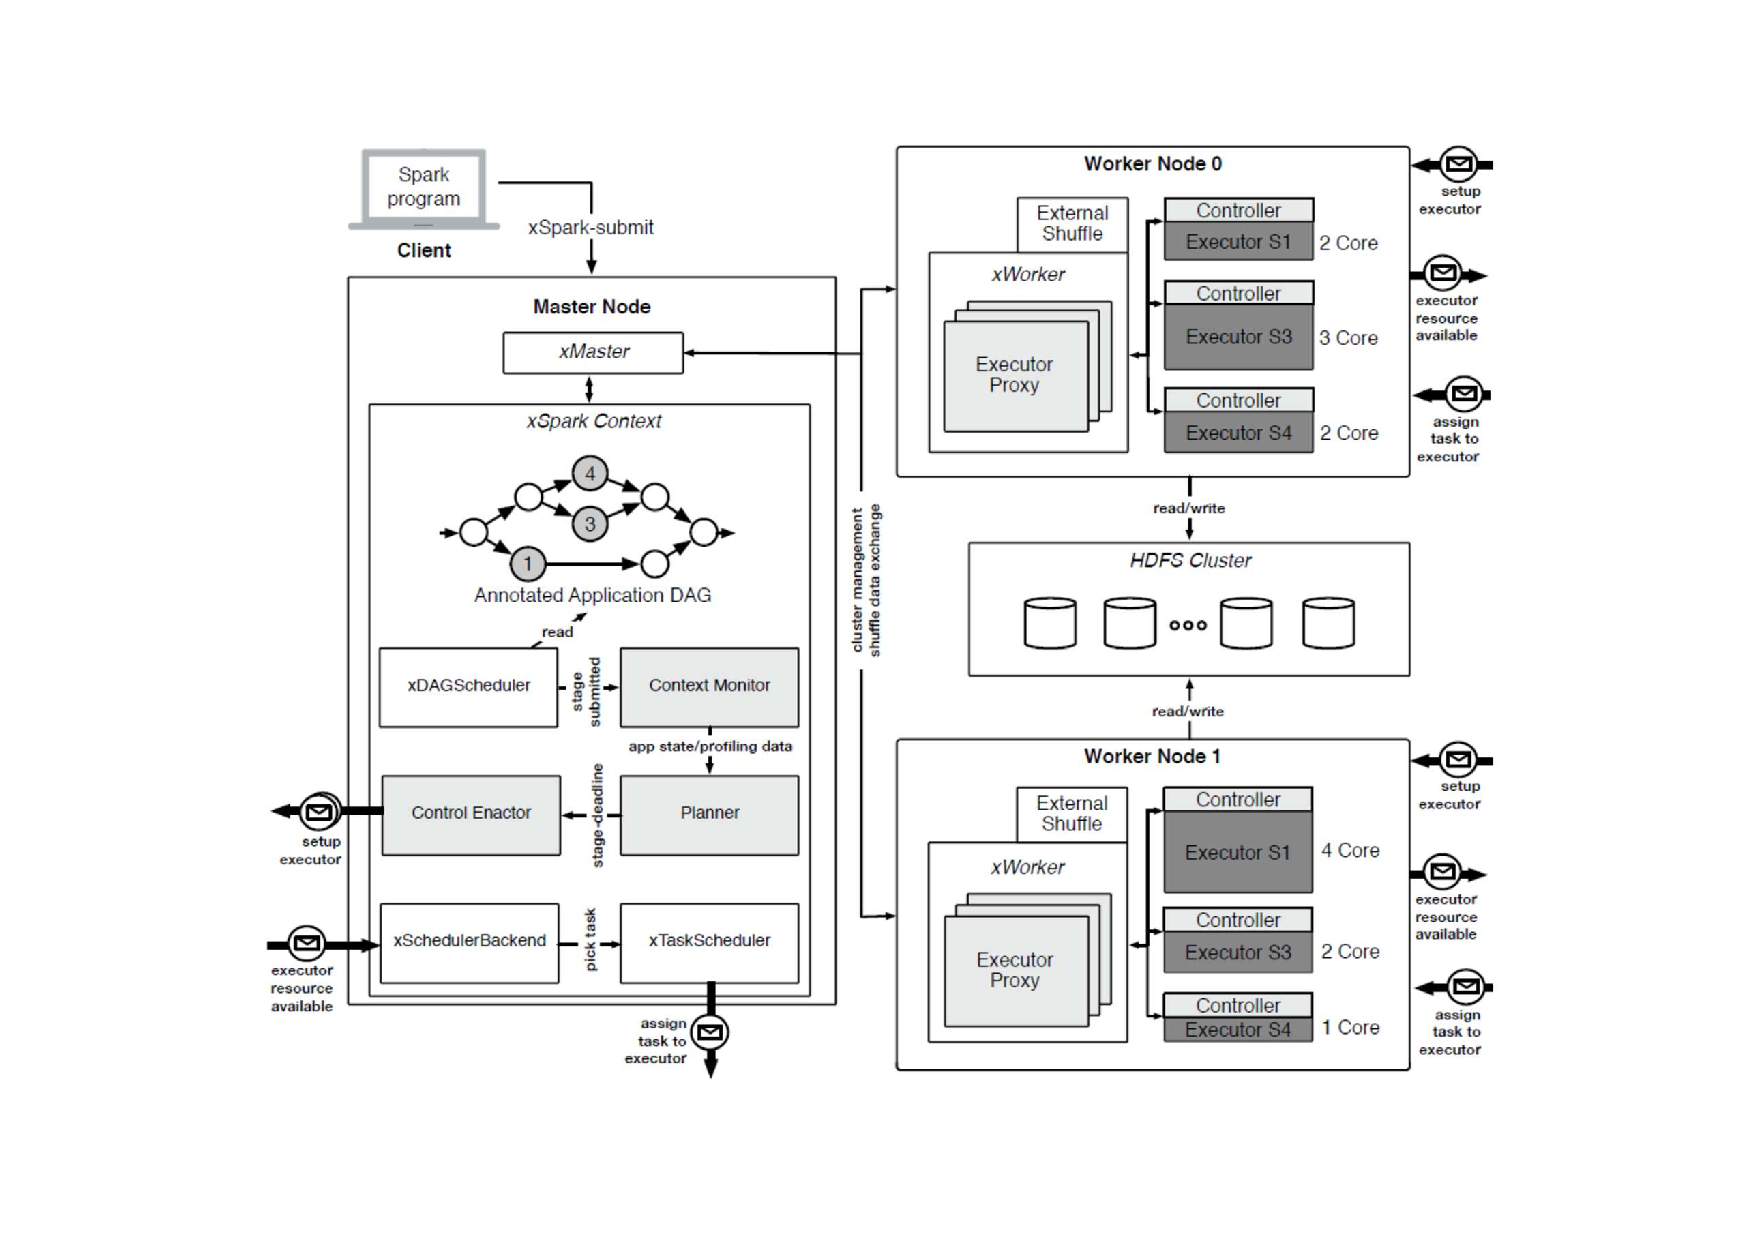
\includegraphics[width=\columnwidth]{Images/xspark_architecture.pdf}  
	\caption[Architecture of xSpark.]{Architecture of xSpark. New components are represented in light grey boxes, meanwhile those that start with an x are the modified ones. In dark grey are represented the containerized components (the executors).}
	\label{fig:xSparkArchitecture}
\end{figure}
\section{Architecture}\label{sec:architecture}

To achieve the objectives of xSpark, the architecture and processing model of Spark have been modified. In Figure 2.2 we can se how xSpark architecture differs from Spark. The principal architectural change introduced by xSpark is an increased focus on stages. Instead of considering entire applications, xSpark reasons on per-stage deadlines. 

xSpark instantiates an executor per stage per worker, instead of a single executor per worker for all the stages that will be executed. This way the resources that are allocated to a single executor only impact the performance of the stages that are associated with it, this leads to a fine grained control over the different stage, and thus on the entire application. When 
multiple stages are run in parallel, multiple executors can be running on the same worker node. When a stage is submitted for execution, one executor per worker is created and bound to that stage. This way computation and data are equally spread across the entire cluster.

Thanks to containers, xSpark can isolate the execution of the different executors that are running on the same worker node and achieve quick, fine-grained resource provisioning. On average, containers can be modified in less than one second, allowing a more precise way of
allocating cores.
Users submit applications and their deadlines to the master node using the submit command. This creates an \textit{xSparkContext} on the master node, containing a\textit{xMaster} object that is used to manage the cluster and that knows all the resources that are available on each worker
node. A \textit{xSparkContext} is composed by six components:
\begin{itemize}
	\item\textit{xDagScheduler} schedules the stages according to the application’s \plan. The submitted stage is enriched with the information obtained during the profiling phase
	\item\textit{ContextMonitor} monitors the progress of the application, taking into account stage scheduling and completion. It also stores information about the performance of the execution, that will be later used to calculate the deadlines and the resources needed by upcoming stages
	\item\textit{Planner} is heuristics based and is used to calculate the deadlines and resources associated with a stage
	\item\textit{ControlEnactor} determines when a stage is ready to be executed, meaning there are enough resources (cores) and sufficient executors become available. It also has the duty of initializing the different executors.
	\item\textit{xSchedulerBackend} controls the stage execution. In particular it launches new tasks by taking into account the resources availability and registers their completion
	\item\textit{xTaskScheduler} also controls stage execution, with the goal of allocating tasks to the available cores to optimize data locality. 
	In general, the closer a data partition required by a task is to the task’s executor, the better.
\end{itemize}

xSpark also modified the worker nodes. Each node contains a \textit{xWorker} that connects to a \textit{xMaster}, generates local controllers for the executors, and controls the evolution of its executor by dynamically scaling their resources. xWorker creates an \textit{Executor Proxy} for each of the executors that are running on its node. These proxies are placed between the executors and the \textit{xSchedulerBackend}, and are used to monitor the execution progress of the stage assigned to the executors. It is important to remember that each executor focuses on a single stage at a time. The heuristic calculates how many tasks must be executed by each of the executors of the same stage, the strategy is to have an equal number of tasks assigned to each of the executors. This way the deadline assigned to each of the executors coincides with the deadline of their stage. This allows the different executors of the same stage to
not be synchronized. Native Spark instead requires that executors with free resources spontaneously require new tasks to execute from the master node. 

Every xWorker uses an External Shuffle Service. Native Spark moves data across the cluster in different ways. If the data is stored on executor’s memory, then the executor itself manages the data exchange. If the data is stored on an external storage system (e.g., HDFS cluster),
they can be retrieved by using different communication protocols. If the data is stored in the internal storage of a worker node, then the data is managed by the External Shuffle Service. Notice that this is not the default, but xSpark adopts this technique to be able to assign
zero CPU cores to an executor, without loosing the ability to read data, since it is effectively not performed by the executor but by the external service.

\section{Heuristic}\label{sec:heuristic}
xSpark uses a heuristic to compute per-stage deadlines and to estimate how many cores must be allocated for a stage to successfully fulfill the deadline. In order to do this, at submission time the user is asked to specify three parameters: i) the application deadline, ii) the cluster size, and iii) the number of cores per worker node. Before executing the application, xSpark performs a feasibility check given the available resources.

When a stage is submitted for execution, its deadline is computed
\[deadline(sk) = \dfrac{\alpha\cdot ApplicationDeadline - SpentTime}{weight(sk)}\]
where $SpentTime$ is the time already spent for execution and $\alpha$ a
value between 0 and 1 that xSpark uses to be more conservative with
respect to the provided ApplicationDeadline. The weight is computed
\[\begin{cases}
w1(sk) = \#(RemainingStages + 1)\\
w2(sk) = \dfrac{{\Sigma}_{{a}_{i=k}}^{k+{w}_{1}}duration(s_i)}{duration(sk)}\\
weight(sk) = \beta\cdot w1(sk) + (1 - \beta) \cdot w2(sk)\\
\end{cases}\]
where w1 is the number of stages still to be scheduled (s included)
and w2 is the rate between the duration of s and the duration of the
remaining stages (s included).
xSpark then proceeds to estimate how many cores are needed to execute the stage:
\[estimatedCores(sk) = \lceil {\dfrac {inputRecords(sk)}{deadline(sk) \cdot nominalRate(sk)}}\rceil\]

where inputRecords is the number of records that will be processed by sk and nominalRate is the number of records processed by a single core per second in stage sk.

Since xSpark controls the resource allocation of a stage before and during the execution, the maximum amount of allocable cores needs to be greater than the estimated one, in order to be able to accelerate when progressing slower than expected 
\[maxAllocableCores(sk) = overscale \cdot estimatedCores(sk)\]
The final step is to determine the initial number of cores that should be assigned to the different executors, xSpark distributes the cores equally amongst the available workers by creating one executor per stage per worker. In this way, it is guaranteed that executor performances will be equal, and that xSpark can compute the same deadline for all the executors. The initial number of cores per executor is computed as
\[initCorePerExec(sk) = \lceil\dfrac {maxAllocableCores(sk)}{overscale \cdot cq \cdot numExecutors}\rceil\cdot cq\]
where $numExecutors$ is the number of executors and $cq$ is the $core\  quantum$, a constant that defines the quantization applied to resource
allocation, the smaller this value is, the more precise the allocation.

\section{Controller}\label{subsec:controller}
Each containerized executor has an associated local controller, whose goal is to fulfill the per-stage deadline taking into account external disturbances by dynamically allocating CPU cores. The controllers use control theory, with no heuristic involved.

The centralized control loop determines the desired stage duration, the maximum and the initial number of cores that should be assigned to the executors and the number of tasks that must be processed. Local controllers adjust the number of allocated cores, according to
the work that has already been accomplished.

Executors that are dedicated to different stages are implicitly independent, and thus their controllers are also independent. The executors that are running in parallel on the same stage must complete the same amount of work (number of tasks) in the same desired time.
This means that local controllers are independent and do not need to communicate among themselves. Moreover, the heuristic is relegated outside the local controller, so that it cannot compromise the controller’s stability.
\begin{figure}
	\centering
	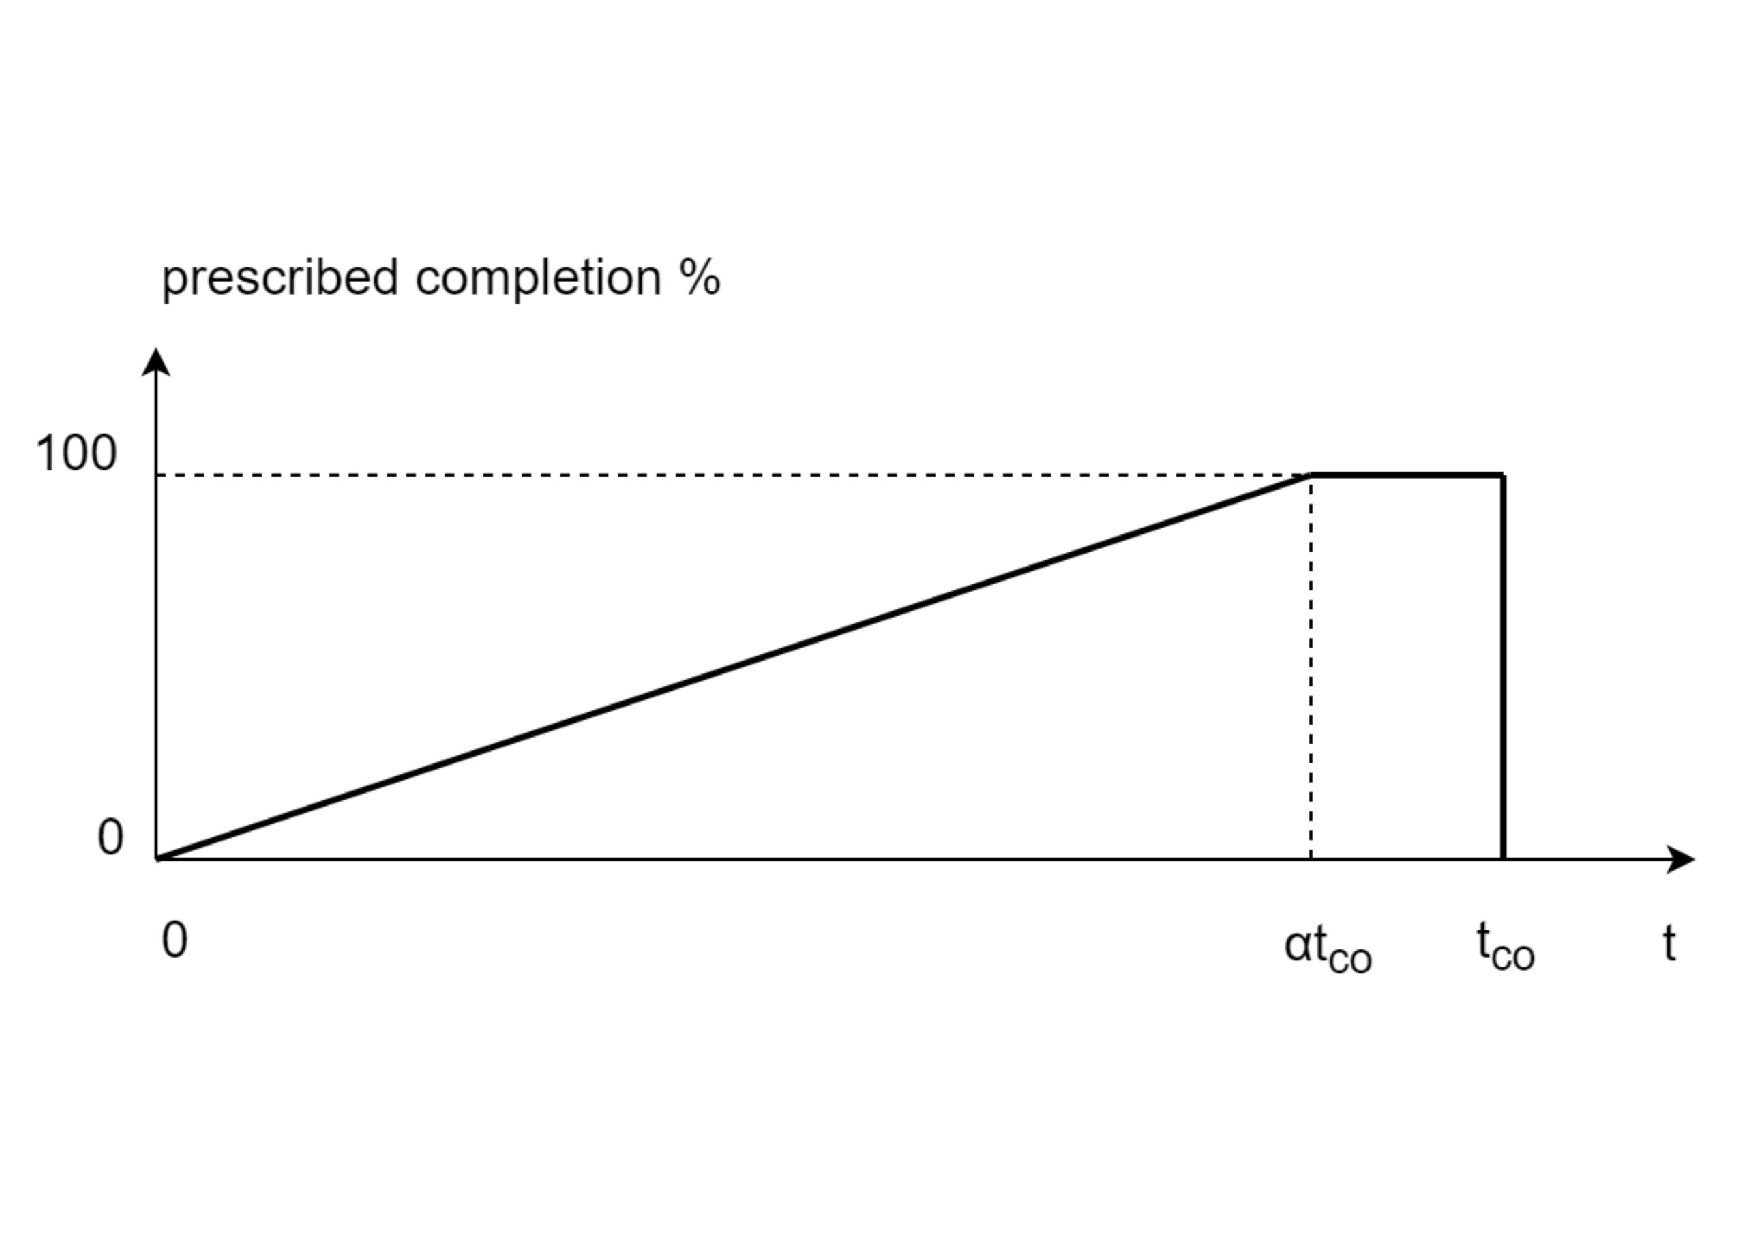
\includegraphics[width=\columnwidth]{Images/exec_controller_set_point.pdf}  
	\caption[Set point generation for an executor controller.]{Set point generation for an executor controller.}
	\label{fig:execControllerSetPoint}
\end{figure}
\begin{figure}
	\centering
	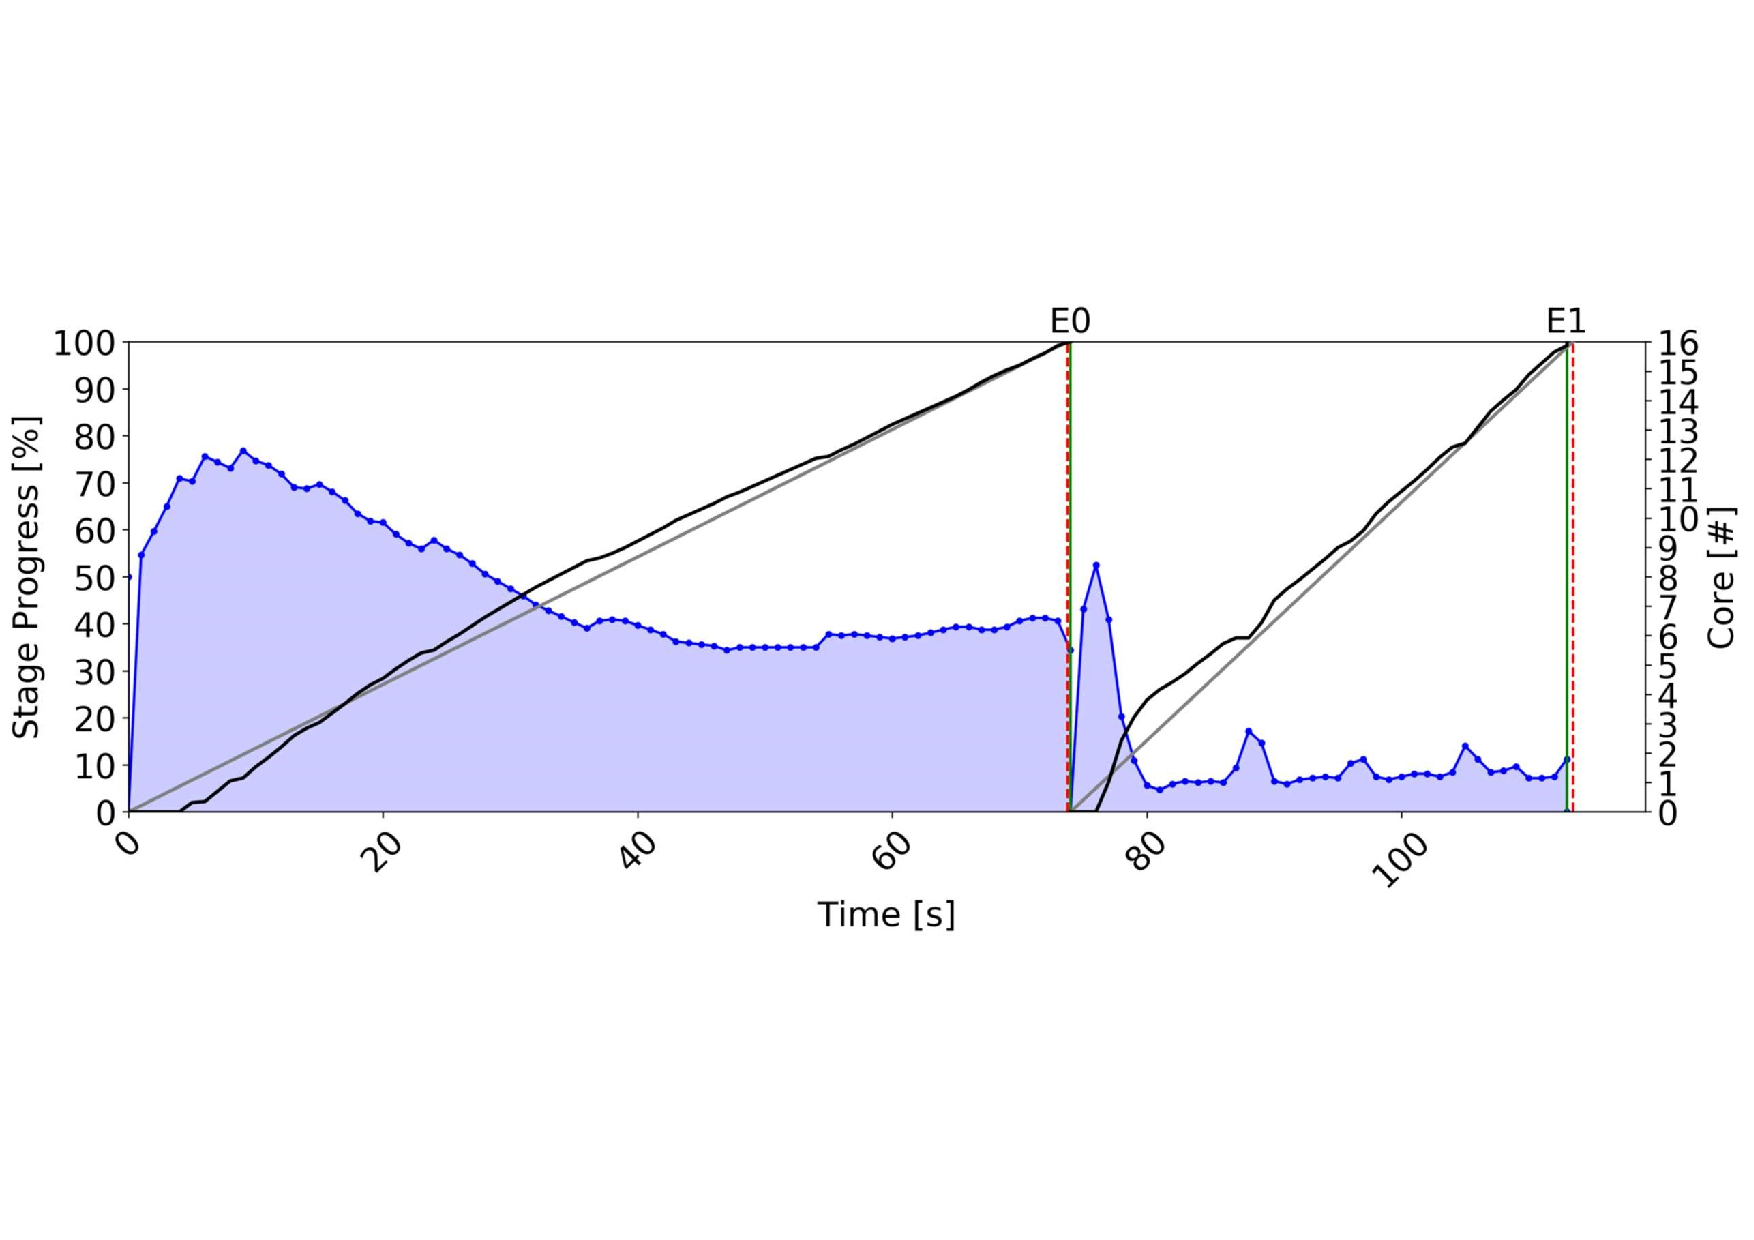
\includegraphics[width=\columnwidth]{Images/xspark_chart_agg_by_key.pdf}  
	\caption[xSpark chart aggrregate-by-key.]{CPU cores allocated to the application aggregate-by-key running on a xSpark worker node. The blue line represents the allocated cores over the time, gray and black line are desired and actual progress rate respectively. Green line represents the obtained stage ending, while dashed red line is the desired one.}
	\label{fig:xsparkChartAggByKey}
\end{figure}

In the controller, the progress set point is chosen based on the desired completion time. Its value is received from the centralized control loop. In \MyFig{fig:execControllerSetPoint} we see the prescribed completion percentage, in particular t\textsubscript{co} is the desired completion time and  $\alpha \in \left(0,1\right]$ is a configuration parameter used to determine how much earlier we are willing to complete the execution with respect to requested deadline,In order to track the set point ramp, we need to use a Proportional plus Integral (PI) controller.
As a result, the discrete-time controller in state space form reads:
\[\begin{cases}
x_{C}(k) = x_{C}(k - 1) + (1 - a)(a _{\%}^{o}(k - 1) - a _{\%}(k - 1))\\
c(k) = Kx_{C}(k) + K(a _{\%}^{o} - a _{\%}(k))\\
\end{cases}\]
where $(a _{\%}^{o}$ is the prescribed progress percentage at each $k$ control
step and a $_{\%}$ is the accomplished completion percent at each $k$ control
step. Notice that it is possible that the controller computes a negative value for $c(k)$, the CPU cores that need to be allocated. To fix this problem $c(k)$ must be clamped between a minimum $_{cmin}$ and a maximum $c_{max}$. To maintain consistency, we need to recompute the state $x_{C}(k)$ as 
\[x_{C}(k) = \dfrac{c(k)}{K} - a _{\%}^{o}(k) + a _{\%}(k)\] 

In \MyFig{fig:xsparkChartAggByKey} the cores allocated to an application executor running
on a worker node are shown. The running application is \textit{aggregateby-
key} and is composed by two stages. The black line represents the
progress of the stage, meanwhile the gray one is the desired progress
rate. The goal of the controller is to reduce the error, i.e., the distance
between the two lines. We want the black line to follow as much as
possible the gray line.
